\documentclass{beamer}\usepackage[]{graphicx}\usepackage[]{color}
%% maxwidth is the original width if it is less than linewidth
%% otherwise use linewidth (to make sure the graphics do not exceed the margin)
\makeatletter
\def\maxwidth{ %
  \ifdim\Gin@nat@width>\linewidth
    \linewidth
  \else
    \Gin@nat@width
  \fi
}
\makeatother

\definecolor{fgcolor}{rgb}{0.345, 0.345, 0.345}
\newcommand{\hlnum}[1]{\textcolor[rgb]{0.686,0.059,0.569}{#1}}%
\newcommand{\hlstr}[1]{\textcolor[rgb]{0.192,0.494,0.8}{#1}}%
\newcommand{\hlcom}[1]{\textcolor[rgb]{0.678,0.584,0.686}{\textit{#1}}}%
\newcommand{\hlopt}[1]{\textcolor[rgb]{0,0,0}{#1}}%
\newcommand{\hlstd}[1]{\textcolor[rgb]{0.345,0.345,0.345}{#1}}%
\newcommand{\hlkwa}[1]{\textcolor[rgb]{0.161,0.373,0.58}{\textbf{#1}}}%
\newcommand{\hlkwb}[1]{\textcolor[rgb]{0.69,0.353,0.396}{#1}}%
\newcommand{\hlkwc}[1]{\textcolor[rgb]{0.333,0.667,0.333}{#1}}%
\newcommand{\hlkwd}[1]{\textcolor[rgb]{0.737,0.353,0.396}{\textbf{#1}}}%
\let\hlipl\hlkwb

\usepackage{framed}
\makeatletter
\newenvironment{kframe}{%
 \def\at@end@of@kframe{}%
 \ifinner\ifhmode%
  \def\at@end@of@kframe{\end{minipage}}%
  \begin{minipage}{\columnwidth}%
 \fi\fi%
 \def\FrameCommand##1{\hskip\@totalleftmargin \hskip-\fboxsep
 \colorbox{shadecolor}{##1}\hskip-\fboxsep
     % There is no \\@totalrightmargin, so:
     \hskip-\linewidth \hskip-\@totalleftmargin \hskip\columnwidth}%
 \MakeFramed {\advance\hsize-\width
   \@totalleftmargin\z@ \linewidth\hsize
   \@setminipage}}%
 {\par\unskip\endMakeFramed%
 \at@end@of@kframe}
\makeatother

\definecolor{shadecolor}{rgb}{.97, .97, .97}
\definecolor{messagecolor}{rgb}{0, 0, 0}
\definecolor{warningcolor}{rgb}{1, 0, 1}
\definecolor{errorcolor}{rgb}{1, 0, 0}
\newenvironment{knitrout}{}{} % an empty environment to be redefined in TeX

\usepackage{alltt}
\usetheme{default}
%\usetheme{Malmoe}

\title[EC999: Quantitative Text Analysis]{EC999: Describing Text} \def\newblock{\hskip .11em plus .33em minus .07em}


\def\Tiny{\fontsize{10pt}{10pt}\selectfont}
\def\smaller{\fontsize{8pt}{8pt}\selectfont}

\institute[Warwick]{University of Chicago \& University of Warwick}
\author[Thiemo Fetzer]{Thiemo Fetzer}

 \date{\today}

\usepackage{natbib}
\usepackage{amsmath}
\usepackage{hyperref}
\usepackage{graphicx}
\usepackage{graphics}

\usepackage{amsfonts}
\usepackage{amssymb}
\usepackage{pdfpages}
\usepackage{natbib}
\usepackage{hyperref}
%\usepackage{enumitem}
 \usepackage{pgffor}
\usepackage{booktabs,caption,fixltx2e}
\usepackage[flushleft]{threeparttable}
\usepackage{verbatim} 
\usepackage{cancel}
\newcommand\xxcancel[1]{\xcancel{#1}\vphantom{#1}}

\usepackage{mathtools,xparse}

\newenvironment{Description}
               {\list{}{\labelwidth=0pt \itemindent-\leftmargin
                        \let\makelabel\Descriptionlabel
                        % or whatever
               }}
               {\endlist}
\newcommand*\Descriptionlabel[1]{%
  \hspace\labelsep
  \normalfont%  reset current font setting
  \color{blue}\bfseries\sffamily% or whatever 
  #1}


\setbeamersize{text margin left = 16pt, text margin right = 16pt}
\newcommand{\code}[1]{\texttt{#1}}

\newenvironment<>{algorithm}[1][\undefined]{%
\begin{actionenv}#2%
\ifx#1\undefined%
   \def\insertblocktitle{Algorithm}%
\else%
   \def\insertblocktitle{Algorithm ({\em#1})}%
\fi%
\par%
\mode<presentation>{%
  \setbeamercolor{block title}{fg=white,bg=yellow!50!black}
  \setbeamercolor{block body}{fg=black,bg=yellow!20}
}%
\usebeamertemplate{block begin}\em}
{\par\usebeamertemplate{block end}\end{actionenv}}


\newenvironment<>{assumption}[1][\undefined]{%
\begin{actionenv}#2%
\ifx#1\undefined%
   \def\insertblocktitle{Assumption}%
\else%
   \def\insertblocktitle{Assumption ({\em#1})}%
\fi%
\par%
\mode<presentation>{%
  \setbeamercolor{block title}{fg=white,bg=blue!50!black}
  \setbeamercolor{block body}{fg=black,bg=blue!20}
}%
\usebeamertemplate{block begin}\em}
{\par\usebeamertemplate{block end}\end{actionenv}}

%changing spacing between knitr code and output
\usepackage{etoolbox} 
\makeatletter 
\preto{\@verbatim}{\topsep=0pt \partopsep=0pt } 
\makeatother
\renewenvironment{knitrout}{\setlength{\topsep}{0mm}}{}
\IfFileExists{upquote.sty}{\usepackage{upquote}}{}
\begin{document}



\AtBeginSection[]
{
 \begin{frame}<beamer>
 \frametitle{Plan}
 \tableofcontents[currentsection]
 \end{frame}
}
\maketitle
 

%%%%%%%%%%%%%%%%%%%%%%%%%%%%




%%%%%%%%%%%%%%%%%%%%%%%%%%%%%%%%%%%%%%%%%%%%%%%%%%%%%%%%%%
\begin{frame}[fragile]{Descriptive Statistics for Text data}
Before performing analysis, you want to get to know your data - this may inform you as to what are the necessary steps for dimensionality reduction. Some simple stats may be...
\begin{Description}
\item[Word (relative) frequency]

\item[Theme (relative) frequency]

\item[Length] in characters, words, lines, sentences, paragraphs, pages, sections, chapters, etc.

\item[Vocabulary diversity] (At its simplest) involves measuring a type-to-token ratio (TTR) where unique words are types and the total words are tokens.

\item[Readability]  Use a combination of syllables and sentence length to indicate ``readability'' in terms of complexity

\item[Formality] Measures relationship of different parts of speech.

\end{Description}
\end{frame}
%%%%%%%%%%%%%%%%%%%%%%%%%%%%%%%%%%%%%%%%%%%%%%%%%%%%%%%%%%%%%%%%%%%%%%%%%


%%%%%%%%%%%%%%%%%%%%%%%%%%%%%%%%%%%%%%%%%%%%%%%%%%%%%%%%%%
\begin{frame}[fragile]{Vocabulary diversity}
 (At its simplest) involves measuring a type-to-token ratio (TTR) where unique words are
types and the total words are tokens. \bigskip

We have already talked about this in the section on Text normalization (pre-processing.)\bigskip

\end{frame}
%%%%%%%%%%%%%%%%%%%%%%%%%%%%%%%%%%%%%%%%%%%%%%%%%%%%%%%%%%%%%%%%%%%%%%%%%






%%%%%%%%%%%%%%%%%%%%%%%%%%%%%%%%%%%%%%%%%%%%%%%%%%%%%%%%%%
\begin{frame}[fragile]{Type-Token Ratio in Congressional speaches}
\begin{knitrout}\tiny
\definecolor{shadecolor}{rgb}{0.969, 0.969, 0.969}\color{fgcolor}\begin{kframe}
\begin{alltt}
\hlstd{dat}
\end{alltt}
\begin{verbatim}
##        Text Types Tokens Sentences   speaker_name speaker_party
## text1 text1  4658  34151      1370     Mike Pence             R
## text2 text2 12509 440340     18343 Bernie Sanders             I
## text3 text3 11849 350175     18239      Rand Paul             R
## text4 text4  8212 182977      8843 Lindsey Graham             R
## text5 text5 10788 270801     12671    Marco Rubio             R
## text6 text6  5003  41051      1613       Jim Webb             D
## text7 text7 12862 304637     14101       Ted Cruz             R
\end{verbatim}
\end{kframe}
\end{knitrout}
$\Rightarrow$ this highlights that there is a negative correlation between the TTR and the total corpus length as measured by the number of sentences. We have seen this previously as \emph{Heap's Law}.  
\end{frame}
%%%%%%%%%%%%%%%%%%%%%%%%%%%%%%%%%%%%%%%%%%%%%%%%%%%%%%%%%%%%%%%%%%%%%%%%%


%%%%%%%%%%%%%%%%%%%%%%%%%%%%%%%%%%%%%%%%%%%%%%%%%%%%%%%%%%
\begin{frame}[fragile]{Alternative Lexical Diversity Measures}
\begin{Description}

\item[TTR] $\frac{\text{total types}}{\text{total tokens}}$

\item[Guiraud] $\frac{\text{total types}}{\sqrt{\text{total tokens}}}$

\item[D] iversity: Randomly sample a fixed number of tokens and count number of types.

\item[MTLD] the mean length of sequential word strings in a text that maintain a given TTR value (McCarthy and Jarvis, 2010) – fixes the TTR at 0.72 and counts the length of the text required to achieve it

\end{Description}

\end{frame}
%%%%%%%%%%%%%%%%%%%%%%%%%%%%%%%%%%%%%%%%%%%%%%%%%%%%%%%%%%%%%%%%%%%%%%%%%



%%%%%%%%%%%%%%%%%%%%%%%%%%%%%%%%%%%%%%%%%%%%%%%%%%%%%%%%%%
\begin{frame}[fragile]{Complexity and Readability}

\begin{itemize}

\item Use of language is endogenous, and electoral incentives may affect the \emph{communication strategies} chosen by elected officials.

\item Readability scores us a combination of syllables and sentence length to indicate ``complexity`` of text

\item  Common in educational research, but could also be used to describe textual complexity and increasingly some political science applications.

\item No natural scale, so most are calibrated in terms of some interpretable metric

\end{itemize}

\begin{center}
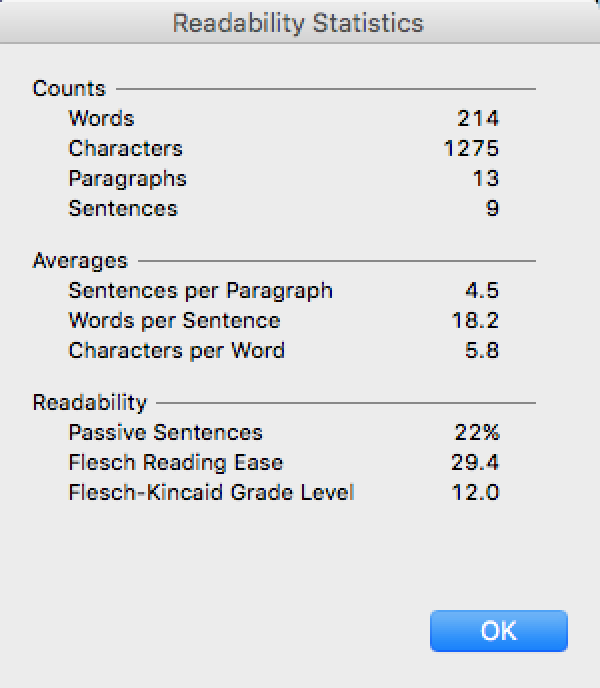
\includegraphics[scale=0.3]{figures/readability.png}
\end{center}

\end{frame}
%%%%%%%%%%%%%%%%%%%%%%%%%%%%%%%%%%%%%%%%%%%%%%%%%%%%%%%%%%%%%%%%%%%%%%%%%




%%%%%%%%%%%%%%%%%%%%%%%%%%%%%%%%%%%%%%%%%%%%%%%%%%%%%%%%%%
\begin{frame}[fragile]{Reading Ease in Congress By Party}

\begin{figure}[h]
\begin{center}
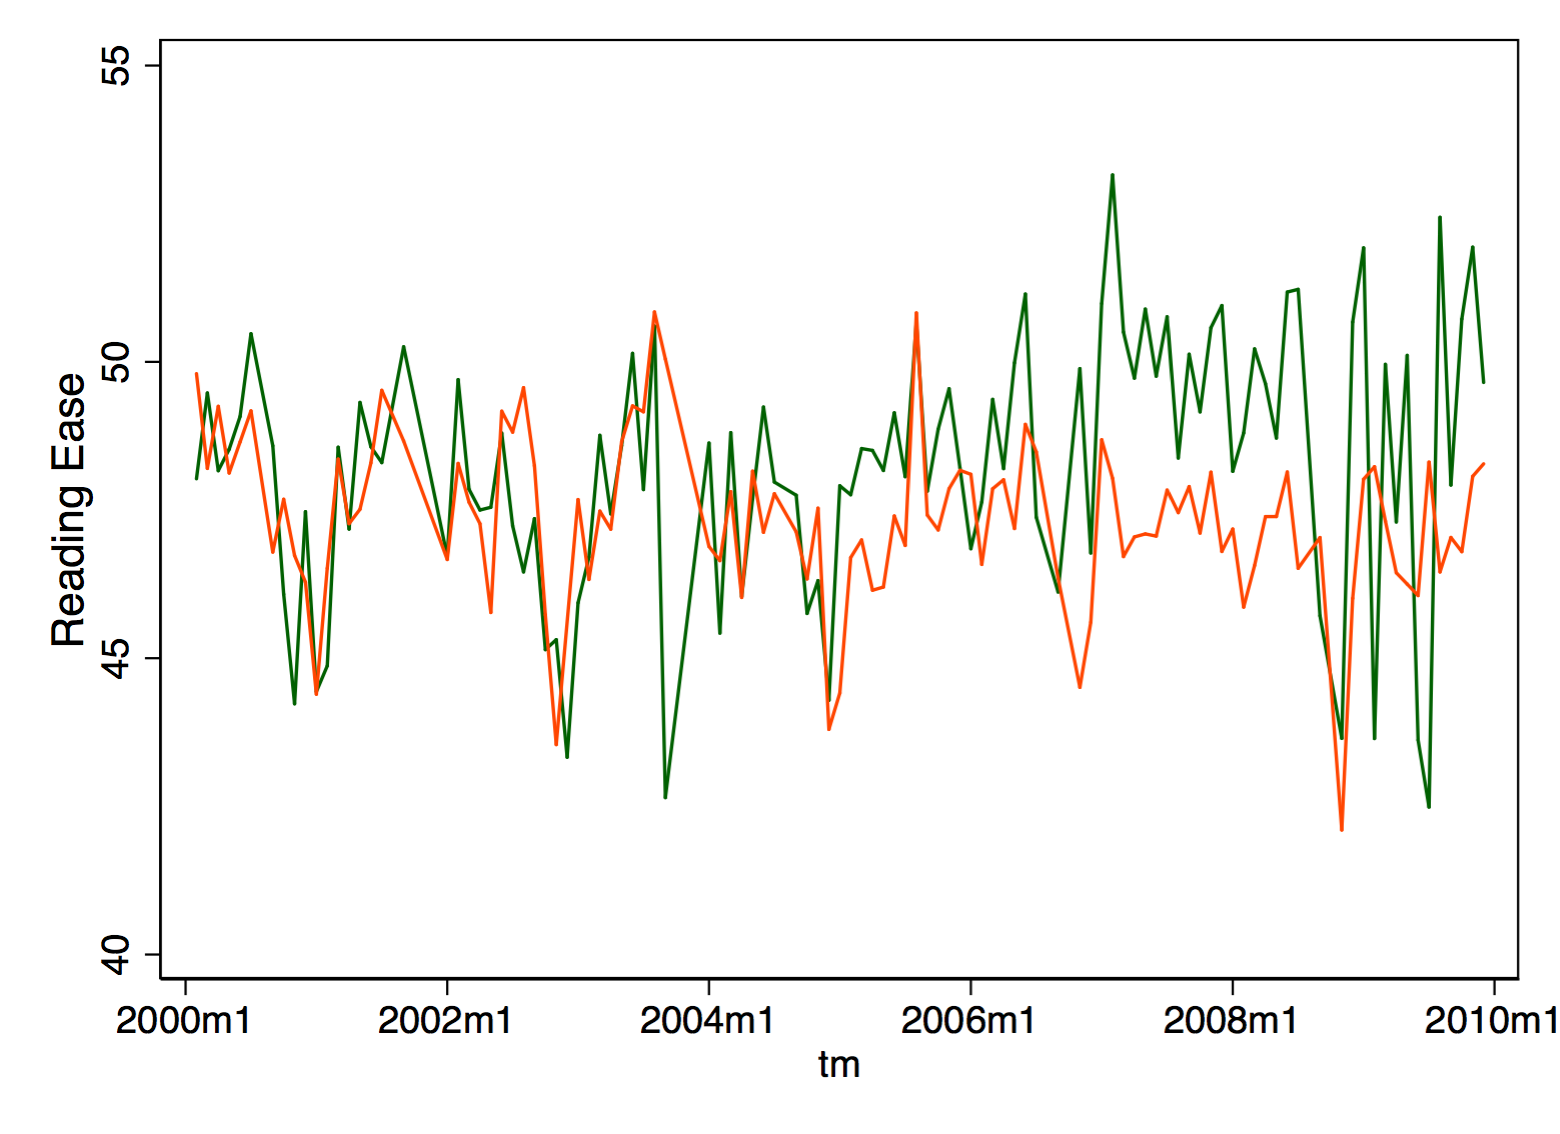
\includegraphics[scale=.29]{figures/reading-ease.png}
\end{center}
\end{figure}

$${\displaystyle 206.835-1.015\left({\frac {\text{total words}}{\text{total sentences}}}\right)-84.6\left({\frac {\text{total syllables}}{\text{total words}}}\right)}$$

$\Rightarrow$ corpus data obtained via the Capitolwords API.
\end{frame}
%%%%%%%%%%%%%%%%%%%%%%%%%%%%%%%%%%%%%%%%%%%%%%%%%%%%%%%%%%%%%%%%%%%%%%%%%


%%%%%%%%%%%%%%%%%%%%%%%%%%%%%%%%%%%%%%%%%%%%%%%%%%%%%%%%%%
\begin{frame}[fragile]{Reading Age in Congress By Part}

\begin{figure}[h]
\begin{center}
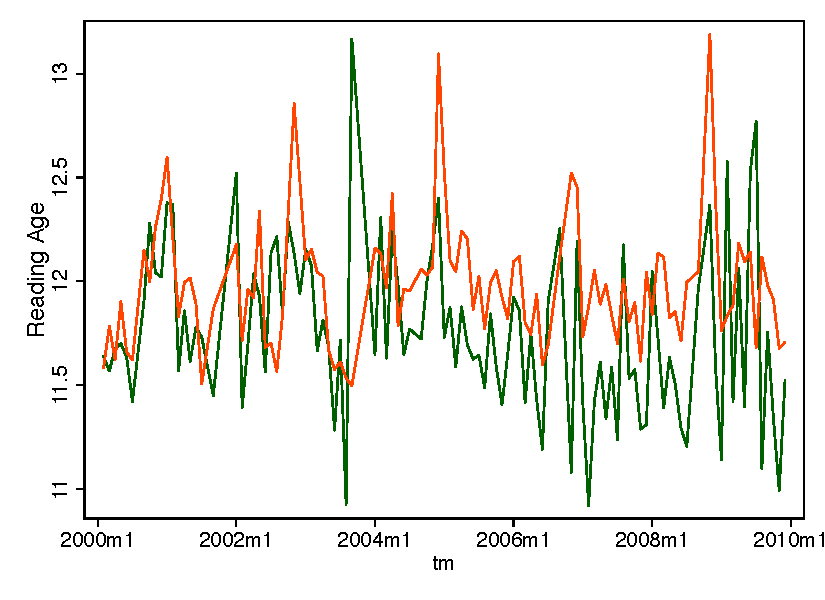
\includegraphics[scale=.56]{figures/reading-age.pdf}
\end{center}
\end{figure}

$$\left({\frac  {{\mbox{total words}}}{{\mbox{total sentences}}}}\right)+11.8\left({\frac  {{\mbox{total syllables}}}{{\mbox{total words}}}}\right)-15.59$$

$\Rightarrow$ corpus data obtained via the Capitolwords API.
\end{frame}
%%%%%%%%%%%%%%%%%%%%%%%%%%%%%%%%%%%%%%%%%%%%%%%%%%%%%%%%%%%%%%%%%%%%%%%%%



%%%%%%%%%%%%%%%%%%%%%%%%%%%%%%%%%%%%%%%%%%%%%%%%%%%%%%%%%%
\begin{frame}[fragile]{Gunning fog index}

\begin{itemize}
\item Measures the readability in terms of the years of formal education required for a person to easily understand the text on first reading

\item  Usually taken on a sample of around 100 words, not omitting any sentences or words
  
\item Computed as 

$$ 0.4 [ ( \frac{\text{total words}}{{\text{total sentences}}} )] + 100 \frac{\text{complex words}}{{\text{total words}}}$$

\item Complex words are defined as those having three or more syllables, not including proper nouns (for example, Ljubljana), familiar jargon or compound words, or counting common suffixes such as -es, -ed, or -ing as a syllable.

\item in $R$ all readability features are embedded in the \code{quanteda} function \code{readability()}.
  
\end{itemize}
\end{frame}
%%%%%%%%%%%%%%%%%%%%%%%%%%%%%%%%%%%%%%%%%%%%%%%%%%%%%%%%%%%%%%%%%%%%%%%%%


%%%%%%%%%%%%%%%%%%%%%%%%%%%%%%%%%%%%%%%%%%%%%%%%%%%%%%%%%%
\begin{frame}[fragile]{Example Readability computation}

\begin{knitrout}\tiny
\definecolor{shadecolor}{rgb}{0.969, 0.969, 0.969}\color{fgcolor}\begin{kframe}
\begin{alltt}
\hlkwd{class}\hlstd{(CORPUS.COMBINED)}
\end{alltt}
\begin{verbatim}
## [1] "corpus" "list"
\end{verbatim}
\begin{alltt}
\hlcom{# can compute various readability indices on a corpus index in quanteda package}
\hlstd{TEMP} \hlkwb{<-} \hlkwd{readability}\hlstd{(CORPUS.COMBINED,} \hlkwc{measure} \hlstd{=} \hlstr{"Flesch.Kincaid"}\hlstd{)}
\hlstd{TEMP}
\end{alltt}
\begin{verbatim}
## text1 text2 text3 text4 text5 text6 text7 
## 11.50 10.57  8.32  9.02  9.32 12.21 10.03
\end{verbatim}
\begin{alltt}
\hlcom{# can add this as piece of meta information}
\hlstd{CORPUS.COMBINED[[}\hlstr{"readability"}\hlstd{]]} \hlkwb{<-} \hlstd{TEMP}

\hlkwd{summary}\hlstd{(CORPUS.COMBINED)}
\end{alltt}
\begin{verbatim}
## Corpus consisting of 7 documents.
## 
##   Text Types Tokens Sentences   speaker_name speaker_party readability
##  text1  4658  34151      1370     Mike Pence             R       11.50
##  text2 12509 440340     18343 Bernie Sanders             I       10.57
##  text3 11849 350175     18239      Rand Paul             R        8.32
##  text4  8212 182977      8843 Lindsey Graham             R        9.02
##  text5 10788 270801     12671    Marco Rubio             R        9.32
##  text6  5003  41051      1613       Jim Webb             D       12.21
##  text7 12862 304637     14101       Ted Cruz             R       10.03
## 
## Source:  /Users/thiemo/Dropbox/Teaching/Quantitative Text Analysis/Week 2d/* on x86_64 by thiemo
## Created: Mon Nov 21 16:25:05 2016
## Notes:
\end{verbatim}
\end{kframe}
\end{knitrout}


\end{frame}
%%%%%%%%%%%%%%%%%%%%%%%%%%%%%%%%%%%%%%%%%%%%%%%%%%%%%%%%%%%%%%%%%%%%%%%%%



%%%%%%%%%%%%%%%%%%%%%%%%%%%%%%%%%%%%%%%%%%%%%%%%%%%%%%%%%%
\begin{frame}[fragile]{Formality Score}
Language is considered more formal when it contains much of the information directly in the text, whereas, contextual language relies on shared experiences to more efficiently dialogue with others.\smallskip

A candidate measure is the Heylighen \& Dewaele's (1999) F-measure. \smallskip

$$F = 50(\frac{nf - nc}{N}+1)$$

Where:

\begin{itemize}

\item $f =  \text{\{noun, adjective, preposition, article\}}$

\item $c = \text{\{pronoun, verb, adverb, interjection\}}$

\item $N = nf + nc$

\end{itemize}

This yields an F-measure between 0 and 100\%, with completely contextualized language on the zero end and completely formal language on the 100 end.

As is evident, this requires known \emph{Parts of Speech}.

\end{frame}
%%%%%%%%%%%%%%%%%%%%%%%%%%%%%%%%%%%%%%%%%%%%%%%%%%%%%%%%%%%%%%%%%%%%%%%%%


%%%%%%%%%%%%%%%%%%%%%%%%%%%%%%%%%%%%%%%%%%%%%%%%%%%%%%%%%%
\begin{frame}[fragile]{Computing Formality Scores in R}


\begin{knitrout}\tiny
\definecolor{shadecolor}{rgb}{0.969, 0.969, 0.969}\color{fgcolor}\begin{kframe}
\begin{alltt}
\hlcom{# installing the formality package which is in developmental state}
\hlkwa{if} \hlstd{(}\hlopt{!}\hlkwd{require}\hlstd{(}\hlstr{"pacman"}\hlstd{))} \hlkwd{install.packages}\hlstd{(}\hlstr{"pacman"}\hlstd{)}
\hlstd{pacman}\hlopt{::}\hlkwd{p_load_gh}\hlstd{(}\hlkwd{c}\hlstd{(}\hlstr{"trinker/formality"}\hlstd{))}
\hlkwd{library}\hlstd{(formality)}
\hlkwd{data}\hlstd{(presidential_debates_2012)}
\hlstd{debateformality} \hlkwb{<-} \hlkwd{formality}\hlstd{(presidential_debates_2012}\hlopt{$}\hlstd{dialogue, presidential_debates_2012}\hlopt{$}\hlstd{person)}
\end{alltt}
\end{kframe}
\end{knitrout}




\end{frame}
%%%%%%%%%%%%%%%%%%%%%%%%%%%%%%%%%%%%%%%%%%%%%%%%%%%%%%%%%%%%%%%%%%%%%%%%%


%%%%%%%%%%%%%%%%%%%%%%%%%%%%%%%%%%%%%%%%%%%%%%%%%%%%%%%%%%
\begin{frame}[fragile]{Some plotting capability}


\begin{knitrout}\tiny
\definecolor{shadecolor}{rgb}{0.969, 0.969, 0.969}\color{fgcolor}\begin{kframe}
\begin{alltt}
\hlkwd{plot}\hlstd{(debateformality)}
\end{alltt}
\end{kframe}

{\centering 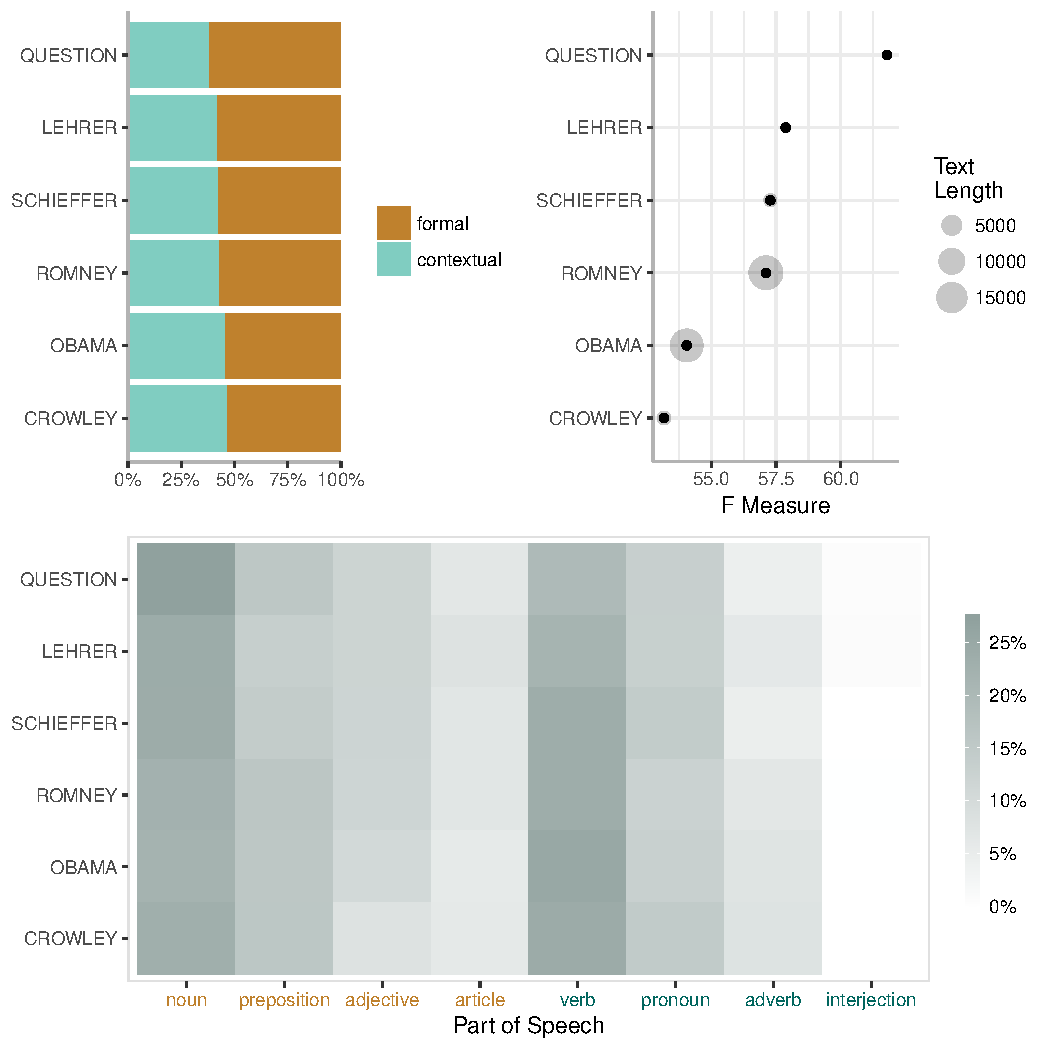
\includegraphics[width=3in]{figures/knitr-formalityplot-1} 

}



\end{knitrout}


\end{frame}
%%%%%%%%%%%%%%%%%%%%%%%%%%%%%%%%%%%%%%%%%%%%%%%%%%%%%%%%%%%%%%%%%%%%%%%%%


\end{document}

